
\begin{figure}
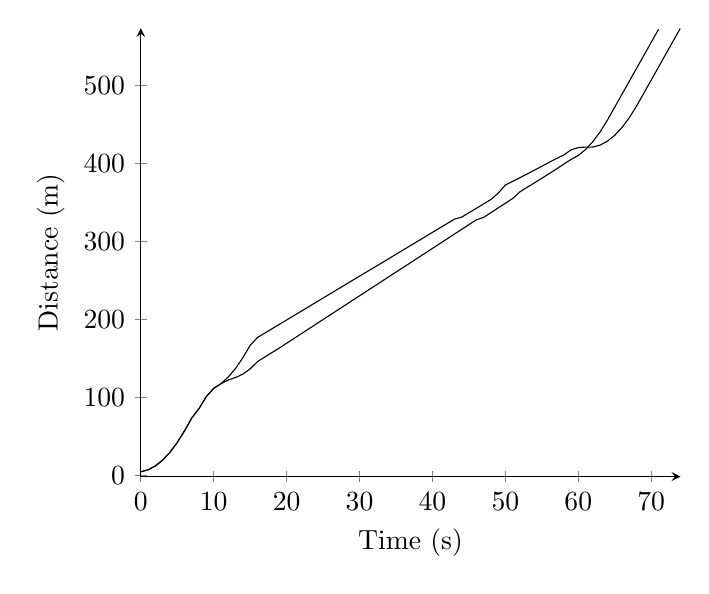
\begin{tikzpicture}
\begin{axis}[
legend style={
	anchor=west
},
axis x line=bottom,
axis y line=left,
ymin=-1,
point meta=explicit symbolic,
xlabel=Time (s),
ylabel=Distance (m)
]
\addplot[] coordinates {
(0, 5.1)
(1, 7.6)
(2, 12.6)
(3, 20.1)
(4, 30.1)
(5, 42.6)
(6, 57.6)
(7, 74.2)
(8, 86.34)
(9, 101.632252112)
(10, 112.059454389)
(11, 118.089689106)
(12, 126.619923822)
(13, 137.650158538)
(14, 151.180393254)
(15, 167.210627971)
(16, 177.240862687)
(17, 182.859590217)
(18, 188.478324971)
(19, 194.097067481)
(20, 199.715818333)
(21, 205.334578174)
(22, 210.953347717)
(23, 216.572127754)
(24, 222.190919166)
(25, 227.809722937)
(26, 233.428540164)
(27, 239.04737208)
(28, 244.666220075)
(29, 250.285085718)
(30, 255.903970788)
(31, 261.522877315)
(32, 267.041807619)
(33, 272.665816528)
(34, 278.289825813)
(35, 283.913835519)
(36, 289.537845698)
(37, 295.161856414)
(38, 300.78586774)
(39, 306.409879764)
(40, 312.033892594)
(41, 317.657906359)
(42, 323.281921215)
(43, 328.90593736)
(44, 331.52995504)
(45, 337.154154506)
(46, 342.778355927)
(47, 348.402559768)
(48, 354.026766649)
(49, 362.15097353)
(50, 372.77518041)
(51, 377.463027468)
(52, 382.152678914)
(53, 386.921797423)
(54, 391.861439847)
(55, 396.80109731)
(56, 401.740782176)
(57, 406.68052661)
(58, 411.147316026)
(59, 417.758113292)
(60, 420.685746825)
(61, 421.361901264)
(62, 421.399879803)
(63, 423.937858341)
(64, 428.975836879)
(65, 436.513815417)
(66, 446.551793955)
(67, 459.089772493)
(68, 474.127751031)
(69, 490.727751031)
(70, 507.327751031)
(71, 523.927751031)
(72, 540.527751031)
(73, 557.127751031)
(74, 573.727751031)
};
\addplot[] coordinates {
(0, 5.1)
(1, 7.6)
(2, 12.6)
(3, 20.1)
(4, 30.1)
(5, 42.6)
(6, 57.6)
(7, 74.2)
(8, 86.34)
(9, 101.632252112)
(10, 112.059454389)
(11, 118.089689106)
(12, 122.659205505)
(13, 125.980175419)
(14, 130.325649848)
(15, 137.088218085)
(16, 146.310975035)
(17, 152.208868611)
(18, 158.010823794)
(19, 163.7651455)
(20, 169.849563772)
(21, 175.933989263)
(22, 182.018422518)
(23, 188.102864142)
(24, 194.1873148)
(25, 200.271775232)
(26, 206.356246262)
(27, 212.440728807)
(28, 218.525223895)
(29, 224.609732678)
(30, 230.694256455)
(31, 236.778796694)
(32, 242.863355063)
(33, 248.947933461)
(34, 255.032534062)
(35, 261.117159369)
(36, 267.101812273)
(37, 273.19196898)
(38, 279.282126129)
(39, 285.37228378)
(40, 291.462442003)
(41, 297.552600881)
(42, 303.642760514)
(43, 309.732921023)
(44, 315.823082559)
(45, 321.913245305)
(46, 328.003409496)
(47, 331.093575427)
(48, 337.183937283)
(49, 343.274301423)
(50, 349.36466844)
(51, 355.455039149)
(52, 364.045409858)
(53, 369.822077205)
(54, 375.600361033)
(55, 381.380996621)
(56, 387.214333609)
(57, 393.315462999)
(58, 399.416618543)
(59, 405.517833001)
(60, 410.631158515)
(61, 418.24448403)
(62, 428.357809544)
(63, 440.971135058)
(64, 456.084460573)
(65, 472.684460573)
(66, 489.284460573)
(67, 505.884460573)
(68, 522.484460573)
(69, 539.084460573)
(70, 555.684460573)
(71, 572.284460573)
};

\end{axis}
\end{tikzpicture}
\label{tik:50:19_O, 19_O.-60, 17_N, 15_S, 15_S.-30, 13_N, 13_N.-40, 12_V}
\caption{50 percent diving with GSC on route $19_O, 19_O.-60, 17_N, 15_S, 15_S.-30, 13_N, 13_N.-40, 12_V$}
\end{figure}
